\documentclass{article}

\usepackage{graphicx}
\usepackage{tikz}
\usepackage{tikzsymbols}
\usetikzlibrary{calc,patterns,shapes.geometric}
\pagestyle{empty}
\usepackage[margin=0pt]{geometry}
\geometry{papersize={14in,12in}}

\def\centerarc[#1](#2)(#3:#4:#5){\draw[#1] ($(#2)+({#5*cos(#3)},{#5*sin(#3)})$) arc (#3:#4:#5);}

\begin{document}
	\begin{figure}
		\centering
		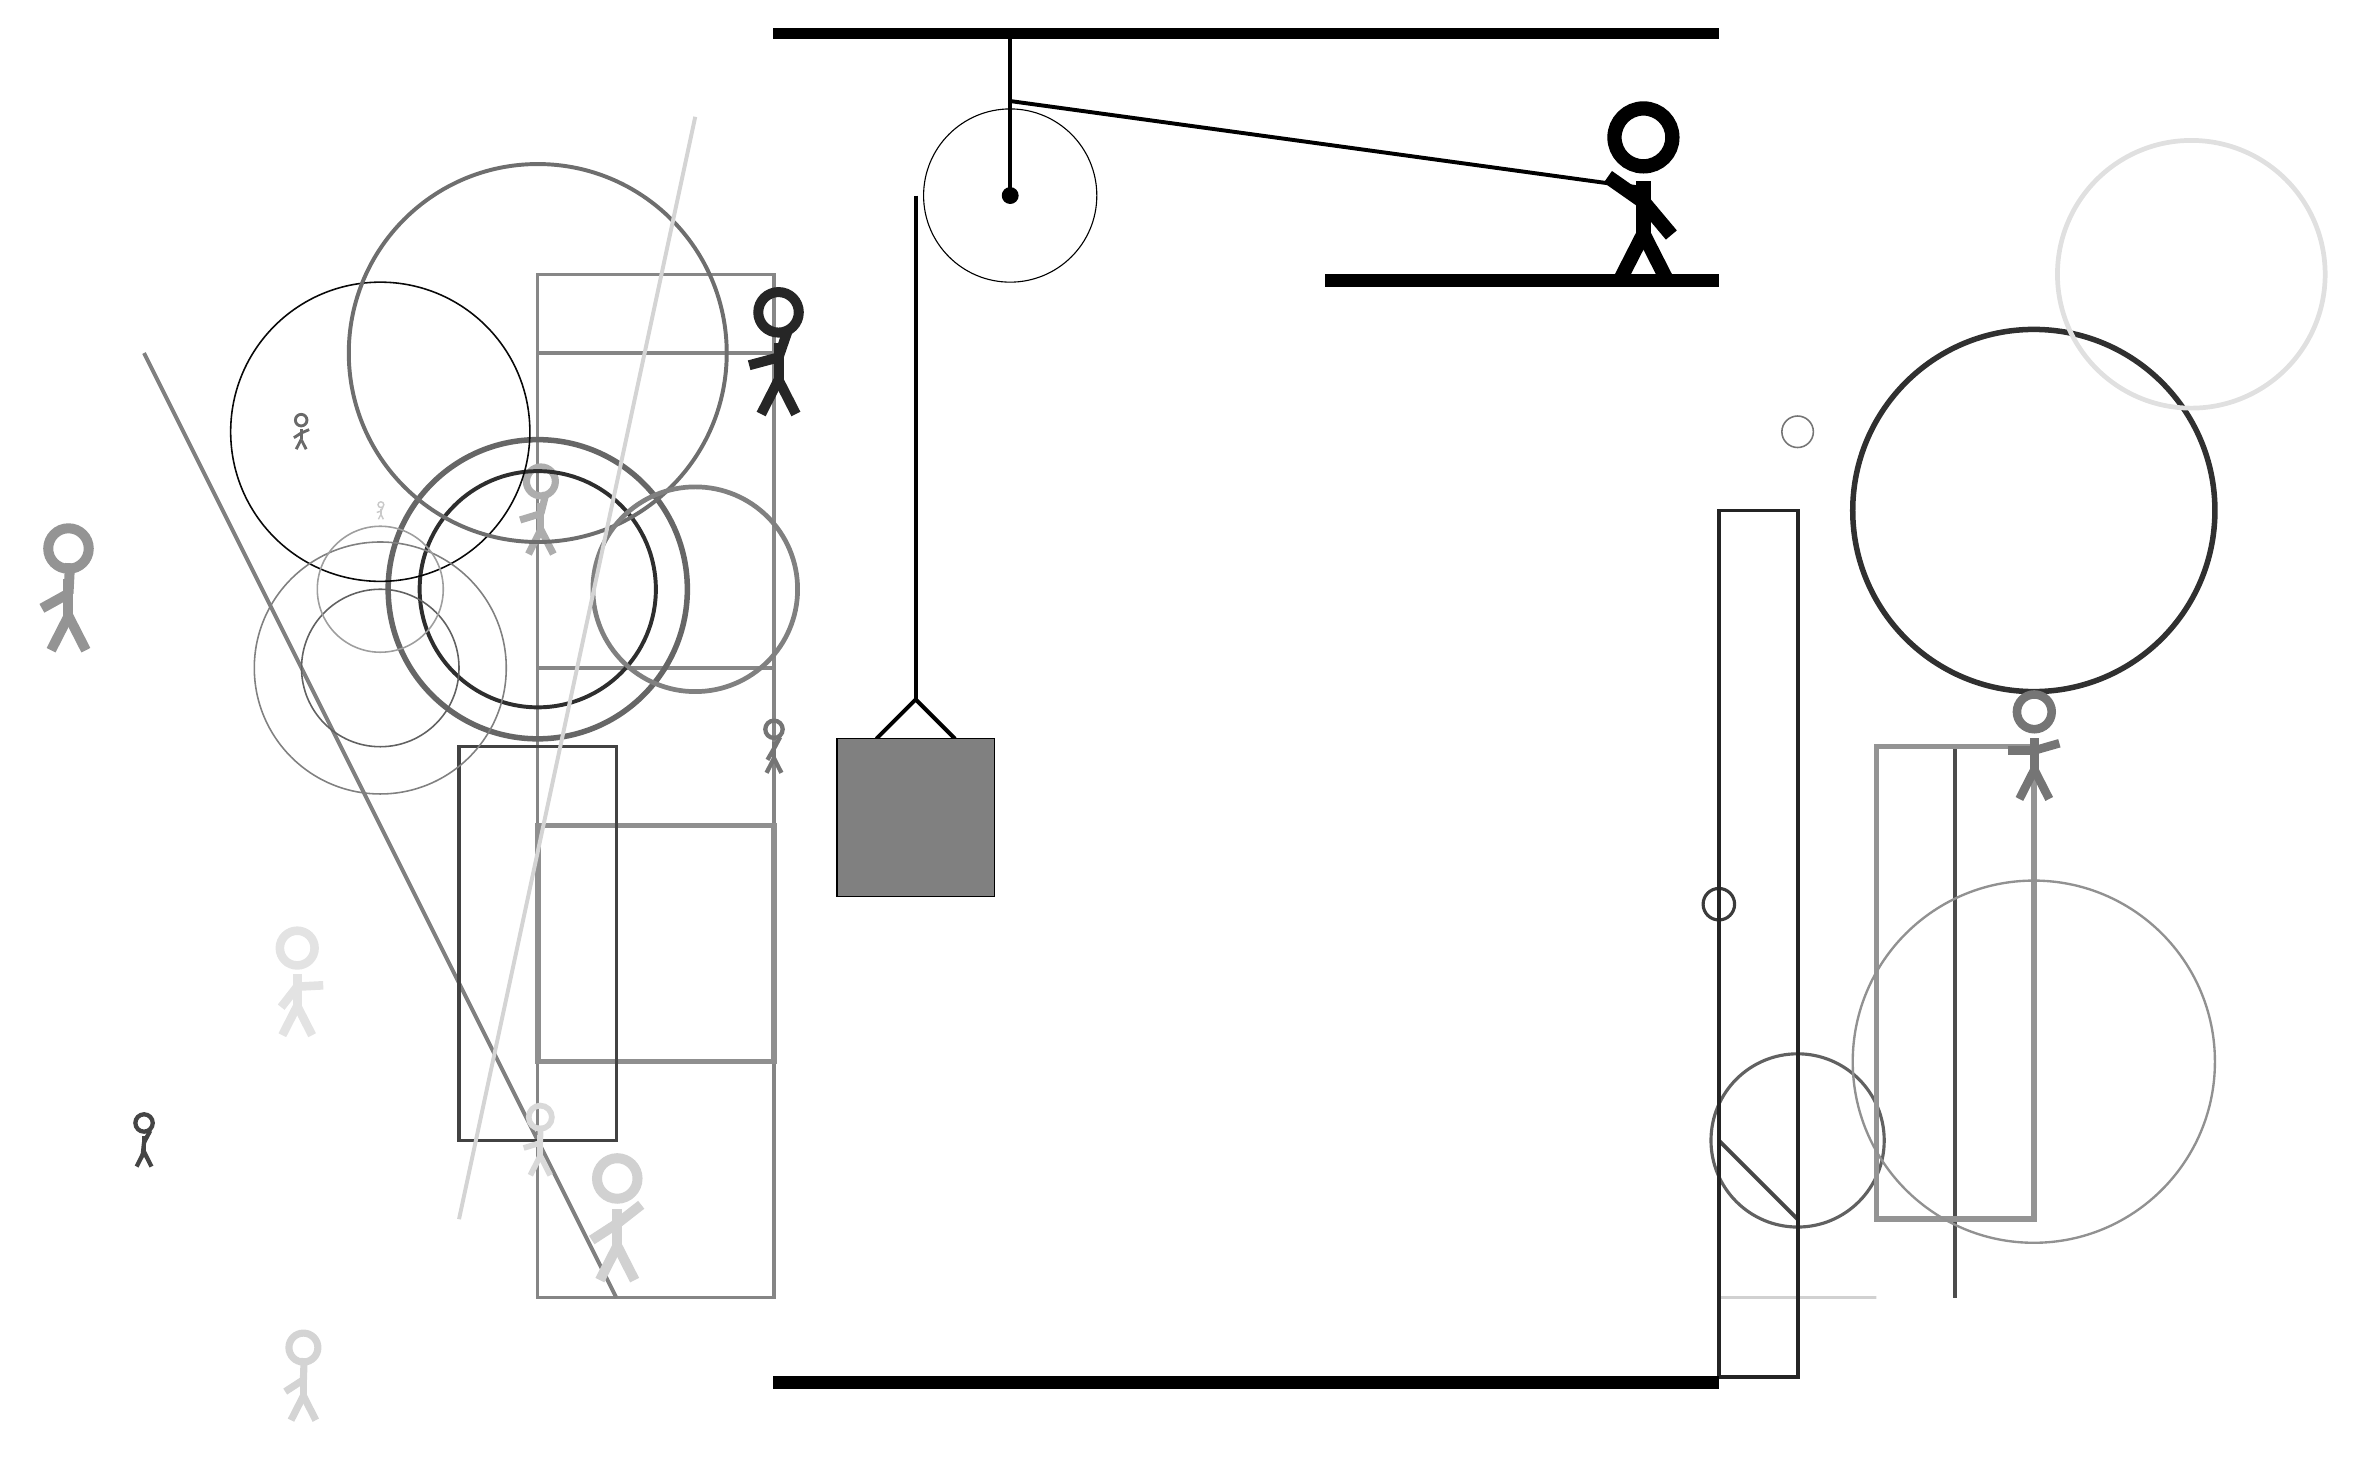
\begin{tikzpicture}
			%%%%% START %%%%%
			
			\draw[fill=black] (-2, 14) rectangle (10, 14.125);
			
			\draw (1, 12) circle (1.1);
			\draw[fill=black] (1, 12) circle (0.1);
			\draw[line width=0.5mm] (1, 14) -- (1, 12);
			
			\draw[line width=0.5mm](-0.7, 5.1) --  (-0.2, 5.6) -- (0.3, 5.1);
			\draw[fill=black!50] (-1.2, 5.1) rectangle (0.8, 3.1);
			
			\draw[line width=0.5mm](-0.2, 12) -- (-0.2, 5.6);
			\centerarc[line width=0.5mm](1, 12)(90:180:1.2000000000000002)
			\draw[line width=0.5mm](1, 13.2) -- (9, 12.1);
			
			\node at (9, 12) {\Strichmaxerl[10][-35][-50]};
			\draw[fill=black] (5, 11) rectangle (10, 10.85);
			
			\draw[line width=0.4mm, color=black!48] (-2, 10) rectangle (-5, -2);
			
			\draw[line width=0.4mm, color=black!47] (-2, 11) rectangle (-5, 6);
			\draw[line width=0.5mm, color=black!50](-4, -2) -- (-10, 10);
			\draw [line width=0.7mm, color=black!60](-5, 7) circle (1.9);
			
			\draw [line width=0.2mm, color=black!54](11, 9) circle (0.2);
			\draw[line width=0.7mm, color=black!44] (-2, 4) rectangle (-5, 1);
			\draw [line width=0.7mm, color=black!81](14, 8) circle (2.3);
			\draw[line width=0.4mm, color=black!74] (-4, 5) rectangle (-6, 0);
			\draw [line width=0.4mm, color=black!62](11, 0) circle (1.1);
			
			\node[line width=0.3mm, color=black!15] at (-5, 0) {\Strichmaxerl[4][17][89]};
			\node[line width=0.3mm, color=black!32] at (-5, 8) {\Strichmaxerl[5][17][76]};
			\node[line width=0.7mm, color=black!73] at (-10, 0) {\Strichmaxerl[3][84][62]};
			\draw [line width=0.5mm, color=black!82](-5, 7) circle (1.5);
			\draw [line width=0.2mm, color=black!97](-7, 9) circle (1.9);
			\draw [line width=0.5mm, color=black!57](-5, 10) circle (2.4);
			\node[line width=0.3mm, color=black!11] at (-8, 2) {\Strichmaxerl[6][52][3]};
			\draw[line width=0.5mm, color=black!72](10, 0) -- (11, -1);
			\draw [line width=0.4mm, color=black!77](10, 3) circle (0.2);
			\node[line width=0.5mm, color=black!42] at (-11, 7) {\Strichmaxerl[7][29][87]};
			\node[line width=0.5mm, color=black!18] at (-4, -1) {\Strichmaxerl[7][33][38]};
			\draw [line width=0.2mm, color=black!62](-7, 6) circle (1.0);
			\draw [line width=0.2mm, color=black!50](-7, 6) circle (1.6);
			\node[line width=0.6mm, color=black!85] at (-2, 10) {\Strichmaxerl[7][15][71]};
			\draw[line width=0.4mm, color=black!18] (12, -2) rectangle (10, -2);
			\draw[line width=0.5mm, color=black!70](13, 5) -- (13, -2);
			
			\node[line width=0.6mm, color=black!21] at (-7, 8) {\Strichmaxerl[1][17][63]};
			
			\draw[line width=0.7mm, color=black!42] (12, -1) rectangle (14, 5);
			\node[line width=0.7mm, color=black!17] at (-8, -3) {\Strichmaxerl[5][33][88]};
			
			\node[line width=0.5mm, color=black!54] at (-2, 5) {\Strichmaxerl[3][60][62]};
			\node[line width=0.2mm, color=black!54] at (14, 5) {\Strichmaxerl[6][0][16]};
			\draw [line width=0.6mm, color=black!50](-3, 7) circle (1.3);
			
			\draw [line width=0.3mm, color=black!43](14, 1) circle (2.3);
			\draw [line width=0.2mm, color=black!69](14, 10) circle (0.0);
			\draw [line width=0.6mm, color=black!12](16, 11) circle (1.7);
			\draw [line width=0.2mm, color=black!38](-7, 7) circle (0.8);
			\draw[line width=0.5mm, color=black!86] (11, -3) rectangle (10, 8);
			\node[line width=0.3mm, color=black!59] at (-8, 9) {\Strichmaxerl[2][33][23]};
			\draw[line width=0.5mm, color=black!17](-6, -1) -- (-3, 13);
			
			\draw[fill=black] (-2, -3) rectangle (10, -3.15);
			
			%%%%% END %%%%%
		\end{tikzpicture}
	\end{figure}	
\end{document}